
%%%%%%%%%%%%%%%%%%%%%%%%%%%%%%%%%%  memoria.tex %%%%%%%%%%%%%%%%%%%%%%%%%%%%%%%%%

%%%%% Memoria del Trabajo Academicamente Dirigido: Experiencias con PyCUDA %%%%%%
%%%%% Alejandro Samarin Perez - Sergio Armas Perez - Lionel A. Mena Garcia %%%%%%
\documentclass[twoside]{article}
\usepackage{fontspec}
\usepackage{xunicode}
\usepackage{xltxtra}
\usepackage{graphicx}
\usepackage{anysize}
\marginsize{3cm}{3cm}{1cm}{1cm}

\graphicspath{{imgs/}}

\usepackage{listings}
\usepackage{color}
\lstloadlanguages{Python}
\lstset{
  language=Python,                      % C,Fortran,XML
  basicstyle=\scriptsize,               % Listados en small
  keywordstyle=\color{red},             % Palabras clave en rojo
  identifierstyle=\ttfamily,
  escapeinside={(*@}{@*)},
  commentstyle=\color{blue},            % comentarios en azul
  stringstyle=\color{green},            % cadenas en verde
  showstringspaces=false,
  frame=tb,
  captionpos=t,
  belowcaptionskip=12pt,
  stepnumber=2,                                         % Opciones de lineas y etiquetas
  numberstyle=\scriptsize,
  numbersep=5pt,
  tabsize=1
}


%%%%%%%%%%%%%%%%%%%%%%%%%%%%%%%%%%%%%%%%%%%%

\begin{document}

\title{Experiencias con Python y CUDA en Computación de Altas Prestaciones}

\author{Sergio Armas, %
     Lionel Mena, %
     Alejandro Samarín, % 
     Vicente Blanco%
     \thanks{Dpto. Estadística, I.O. y Computación, Univ. La Laguna, e-mail: {\tt vblanco@ull.es}} ,%
     Alberto Morales y % 
     Francisco Almeida
}

\maketitle
% Oculta las cabeceras y los números de página.
% Ambos elemetos se añadirán durante la edición de las actas completas.
\markboth{}{}
\pagestyle{empty} 
\thispagestyle{empty} % Oculta el número de la primera página

\begin{abstract}
El aprovechamiento de la capacidad de cómputo de los dispositivos gráficos para resolver problemas computacionalmente complejos está en auge. El alto grado de paralelismo que esta arquitectura provee, además de la disponibilidad de kits especializados de desarrollo de software para el público general, abren la puerta a nuevas formas de resolver problemas científicos en una fracción del tiempo que emplearían algoritmos similares basados en CPU. El siguiente paso es encontrar el equilibrio entre la potencia de estos paradigmas de programación y la flexibilidad de los lenguajes modernos. Es aquí donde PyCUDA entra en escena; un "wrapper" de la programación CUDA para Python, de forma que ofrece al programador el acceso a la computación de altas prestaciones sobre dispositivos gráficos sin abandonar la comodidad y el dinamismo de este lenguaje (orientación a objetos, tipado dinámico, intérprete interactivo, etc.). Nuestros objetivos se centran en, por un lado, preparar una máquina de prueba equipada con el hardware necesario y, por otro, comprobar las facilidades que promete PyCUDA así como su rendimiento frente a problemas reales.
\end{abstract}

% \begin{keywords}
% Python, CUDA, 
% \end{keywords}

\section{Introducción}

\ldots utilizando PyCUDA~\cite{DBLP:journals/corr/abs-0911-3456}

y una gráfica \ref{fig:Fermi}

\begin{figure}
	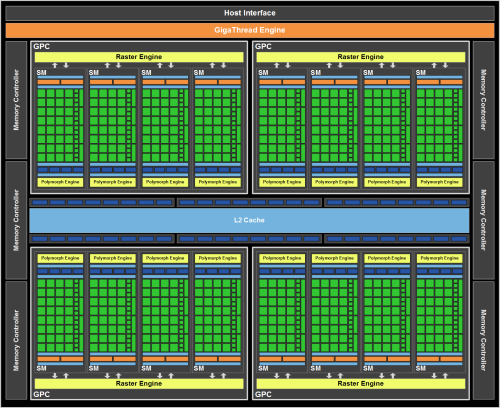
\includegraphics[width=.45\textwidth]{block_diagram_Fermi}
	\caption{\label{fig:Fermi} Diagrama de bloques de una GPU Tesla M2070 (Fermi)}
\end{figure}

y un código \ref{code:filter}

\lstinputlisting[%
   float=t,
   caption={Codigo de filtros en Python},
   label={code:filter} 
   ]%
   {code/filter.py}

\bibliographystyle{Jornadas}
\bibliography{memoria}

\end{document}

